\documentclass[12pt,a4paper]{article}

% Packages
\usepackage[utf8]{inputenc}
\usepackage[T1]{fontenc}
\usepackage{lmodern}
\usepackage[english]{babel}
\usepackage{geometry}
\usepackage{fancyhdr}
\usepackage{hyperref}
\usepackage{listings}
\usepackage{enumitem}
\usepackage{titlesec}
\usepackage{tikz}
\usetikzlibrary{arrows.meta, positioning}

% Page geometry
\geometry{
    a4paper,
    left=2.5cm,
    right=2.5cm,
    top=3cm,
    bottom=3cm
}

% Header and footer
\pagestyle{fancy}
\fancyhf{}
\fancyhead[L]{AI-Assisted Software Development}
\fancyhead[R]{Warrior Race Game Project}
\fancyfoot[C]{\thepage}

% Hyperref setup
\hypersetup{
    colorlinks=true,
    linkcolor=blue,
    urlcolor=blue,
    citecolor=blue,
    pdfauthor={AI Agent Analysis System},
    pdftitle={Reflective Analysis: AI-Assisted Software Development}
}

% Title formatting
\titleformat{\section}{\Large\bfseries}{\thesection}{1em}{}
\titleformat{\subsection}{\large\bfseries}{\thesubsection}{1em}{}
\titleformat{\subsubsection}{\normalsize\bfseries}{\thesubsubsection}{1em}{}

\begin{document}

% Title page
\begin{titlepage}
    \centering
    \vspace*{4cm}
    
    {\Huge\bfseries AI-Assisted Project Development\par}
    
    \vspace{1cm}
    
    {\Large Warrior Race Game Project\par}
    
    \vspace{2cm}
    
    \begin{tabular}{rl}
        \textbf{Author:} & Jacek Ejsmont \\
        \textbf{} & in collaboration with Claude Haiku 4.5 \\
        \textbf{Project:} & Terminal-Based Roguelike Game in C \\
        \textbf{Date:} & January 2026 \\
        \textbf{Active Development:} & November -- December 2025 \\
    \end{tabular}
    
    \vspace{1cm}
\end{titlepage}

% Executive Summary
% \section*{Executive Summary}
% This document provides a comprehensive reflective analysis of the cooperation between a first-year student and artificial intelligence tools during the development of the Warrior Race Game—a terminal-based game implemented in C using the ncurses library. The project successfully leveraged multiple AI technologies (GitHub Copilot Agent with Claude Sonnet 4.5 and GPT-5.1-Codex-Max, ChatGPT, Google Gemini, and others) to achieve rapid development while maintaining high code quality standards and a quick learning curve. The final product comprises approximately 3,300 lines of well-structured C code, organized into modular components with comprehensive functionality, including dynamic enemies, a power-up system, both aggressive and passive obstacles, as well as a ranking mechanism.

% Table of contents
\tableofcontents
\newpage

% Main content
\section{Evolution of AI Cooperation Workflow}

The workflow at the beginning of the project was predominantly traditional, with AI serving as an intelligent autocomplete tool rather than a collaborative partner. \\
A fundamental shift in the cooperation model occured when the developer began using GitHub Copilot in ``Agent mode'' through a pull request workflow. The developer provided structured instructions, project outline, and current development phase. Then, changes were proposed, reviewed, and iteratively refined through PR comments. During this phase, the codebase was restructured into discrete modules. \\
The final evolution phase saw the developer orchestrating multiple AI tools in a sophisticated workflow shown below. The integration of AI tools significantly improved output quality on the first iteration, accelerating development while maintaining code quality.

\subsubsection*{Workflow Characteristics:}

\begin{enumerate}
    \item \textbf{Prompt Engineering Pipeline:}
    \begin{itemize}
        \item ChatGPT/Google Gemini used to create detailed, structured prompts
        \item Prompts included specific technical requirements, code style guidelines, and quality expectations
        \item Example: Instructions screen implementation used Gemini to generate comprehensive implementation requirements
    \end{itemize}
    
    \item \textbf{Specialized Tool Selection:}
    \begin{itemize}
        \item Claude Sonnet 4.5 for feature implementation and refactoring
        \item GPT-5.1-Codex-Max for level design simulation and gameplay balancing
        \item ChatGPT for ideation and conceptual problem-solving
        \item Google Gemini for structured documentation and detailed prompt creation
    \end{itemize}
    
    \item \textbf{Iterative Refinement Cycles:}
    \begin{itemize}
        \item Initial AI implementation rarely met all requirements
        \item Typically required 2--4 refinement cycles per major feature
        \item Developer maintained final authority on code style and architecture decisions
    \end{itemize}
    
    \item \textbf{Quality Assurance Integration:}
    \begin{itemize}
        \item Regular code review requests to AI for bug identification
        \item Comprehensive testing after each major implementation
        \item Manual adjustment of gameplay parameters (timing, balance, visual feedback)
    \end{itemize}
\end{enumerate}

\begin{figure}[ht]
\centering
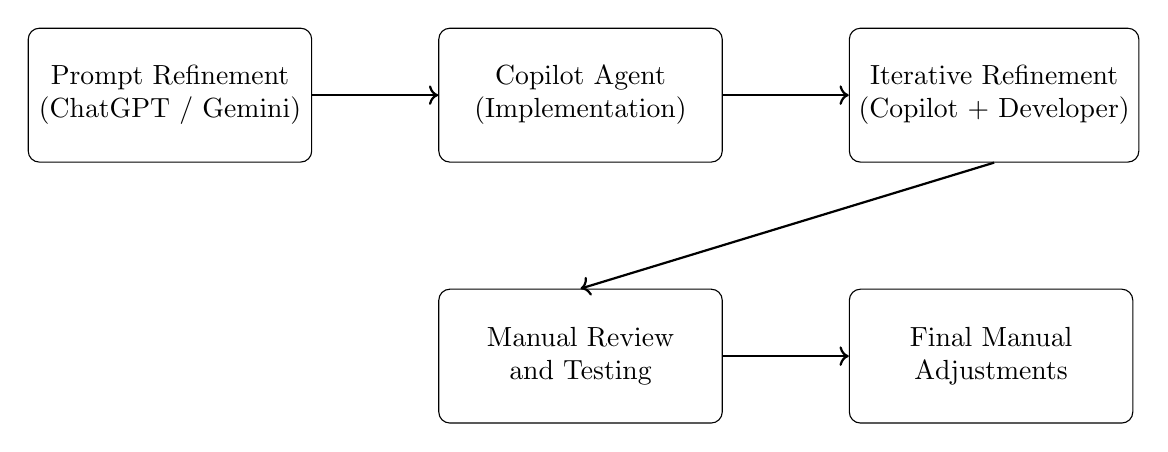
\begin{tikzpicture}[
    node distance=1.6cm,
    every node/.style={
        draw,
        rectangle,
        rounded corners,
        align=center,
        minimum width=3.6cm,
        minimum height=1.7cm
    },
    arrow/.style={->, thick}
]

% Top row
\node (task) {Prompt Refinement\\(ChatGPT / Gemini)};
\node (copilot) [right=of task] {Copilot Agent\\(Implementation)};
\node (iterative) [right=of copilot] {Iterative Refinement\\(Copilot + Developer)};

% Bottom row
\node (review) [below=of copilot] {Manual Review\\and Testing};
\node (final) [right=of review] {Final Manual\\Adjustments};

% Arrows (top row)
\draw[arrow] (task) -- (copilot);
\draw[arrow] (copilot) -- (iterative);

% Transition to second row
\draw[arrow] (iterative.south) -- (review.north);

% Bottom row
\draw[arrow] (review) -- (final);

\end{tikzpicture}
\caption{Final development workflow}
\end{figure}

\newpage

\section{Strengths of AI Collaboration}

\subsection{Accelerated Development Velocity}

The integration of AI tools significantly compressed development timelines while maintaining code quality:

\subsubsection*{Impact and Benefits:}
\begin{itemize}
    \item Complex features (e.g., power-up system with 4 variants, 3 passive obstacle types) implemented in single development sessions
    \item Rapid prototyping of enemy movement algorithms (random walkers, chasers, teleporters) with correct initial implementations
    \item Fast iteration on user interface elements (menu systems, status displays, instructions screen)
\end{itemize}

\subsection{Architectural Consistency and Best Practices}

AI tooling, particularly GitHub Copilot Agent, demonstrated strong capability in maintaining architectural patterns and code conventions, granted that the had the necessary context:

\subsubsection*{Structural Contributions:}
\begin{enumerate}
    \item \textbf{Modular Organization:} Successfully refactored monolithic code into clean module boundaries
    \item \textbf{Memory Management:} Consistent application of allocation/deallocation patterns with proper error checking
    \item \textbf{ncurses Conventions:} Proper window lifecycle management and screen coordinate handling
    \item \textbf{Function Sizing:} Adherence to function length constraints ($\leq$1024 bytes) through appropriate decomposition
    \item \textbf{Standarization:} Uniform naming conventions and error handling patterns across modules
\end{enumerate}

\subsection{Security and Robustness}

AI-assisted development included proactive identification of security vulnerabilities and robustness issues:

\subsubsection*{Security Contributions:}
\begin{itemize}
    \item Buffer overflow prevention through consistent use of bounded string operations (\texttt{strncpy} with manual null termination)
    \item Input validation for all file parsing operations
    \item Bounds checking before array access
    \item Memory leak detection and resolution
\end{itemize}

\subsubsection*{Robustness Enhancements:}
\begin{itemize}
    \item Comprehensive null pointer checks before dereference operations
    \item Graceful degradation when resources unavailable (e.g., file not found scenarios)
    \item Proper cleanup in error paths
    \item Frame rate consistency through careful timing management
\end{itemize}

\subsection{Comprehensive Implementation Coverage}

AI tools excelled at generating complete, feature-rich implementations:

\subsubsection*{Feature Completeness:}
\begin{enumerate}
    \item \textbf{Power-Up System:}
    \begin{itemize}
        \item Four distinct power-up types with unique visual indicators
        \item Time-based effect management with proper state restoration
        \item User interface integration showing active effects
        \item Collision detection and pickup mechanics
    \end{itemize}
    
    \item \textbf{Ranking System:}
    \begin{itemize}
        \item Score calculation with multiple factors (totems, time, lives)
        \item Persistent storage with human-readable format
        \item Per-level leaderboards with top-10 tracking
        \item Integration with menu system for viewing
    \end{itemize}
    
    \item \textbf{Aggressive Obstacles:}
    \begin{itemize}
        \item Time-based activation cycles
        \item Directional damage mechanics
        \item Visual state indicators
        \item Configurable parameters per instance
    \end{itemize}
\end{enumerate}

\subsection{Cross-Domain Knowledge Integration}

AI tools provided valuable assistance beyond pure code generation:

\subsubsection*{Documentation and Communication:}
\begin{itemize}
    \item Clear code comments explaining complex algorithms
    \item Well-structured prompts for subsequent AI interactions
    \item Comprehensive error messages for debugging
    \item User experience considerations (keybind conventions, menu navigation patterns)
\end{itemize}

\subsubsection*{Algorithm Implementation:}
\begin{itemize}
    \item Pathfinding logic for chaser enemies
    \item Random walk algorithms with boundary constraints
    \item Teleportation mechanics with collision avoidance
    \item State machine implementations for enemy behaviors
\end{itemize}

\newpage

\section{Current Weaknesses and Limitations}

\subsection{Contextual Understanding Limitations}

Despite sophisticated capabilities, AI tools exhibited consistent limitations in maintaining project-wide context:

\subsubsection*{Manifestations:}
\begin{enumerate}
    \item \textbf{Style Inconsistencies:} Initial implementations often deviated from established code style despite explicit instructions in \texttt{copilot-instructions.md}

    \item \textbf{Legacy Code Integration:} AI tools sometimes ignored, duplicated or even conflicted with existing abstractions
    
    \item \textbf{Implicit Requirements:} AI tools struggled with unstated expectations based on project conventions
    \begin{itemize}
        \item Manual review consistently needed to ensure adherence to implicit coding standards
        \item Multiple refinement cycles necessary to achieve desired code organization
    \end{itemize}
\end{enumerate}

\subsubsection*{Developer Reflection:}
\begin{quote}
``There were some issues with the initial implementation, so I had to rework parts of it manually. The implementation of new window management just wasn't in line with the existing code style and structure.'' (December 11, 2025)
\end{quote}

\subsection{Creative and Aesthetic Judgment}

AI tools demonstrated significant limitations in subjective design decisions:

\subsubsection*{Level Design Challenges:}
\begin{itemize}
    \item Generated level layouts were functionally correct but lacked engaging gameplay flow
    \item Entity placement was mechanically valid but strategically uninteresting
    \item Difficulty curves were inconsistent (or outright non-existent) across AI-generated levels
\end{itemize}

\subsubsection*{User Interface Aesthetics:}
\begin{itemize}
    \item Initial menu layouts had required manual redesign for visual appeal
    \item Color scheme choices sometimes prioritized convention over aesthetics
    \item Enemy movement speeds, power-up durations and aggressive obstacle timings needed manual tuning for fairness and a smooth game experience
    \item Score calculation weights required developer judgment
\end{itemize}

\subsection{Iterative Refinement Requirement}

A consistent pattern emerged in which AI implementations required multiple refinement cycles:

\subsubsection*{Typical Refinement Pattern:}
\begin{enumerate}
    \item \textbf{Initial Implementation (70--80\% correct):}
    \begin{itemize}
        \item Core functionality implemented
        \item Integration issues present
        \item Edge cases sometimes overlooked
    \end{itemize}
    
    \item \textbf{First Refinement (80--90\% correct):}
    \begin{itemize}
        \item Integration issues resolved
        \item Most edge cases handled
        \item Style inconsistencies remain
    \end{itemize}
    
    \item \textbf{Second Refinement (90--95\% correct):}
    \begin{itemize}
        \item Style consistency achieved
        \item Minor edge cases and bugs present
    \end{itemize}
    
    \item \textbf{Manual Finalization (95--100\%):}
    \begin{itemize}
        \item Final style and balance adjustments
        \item Subtle interaction improvements
        \item Documentation completion
    \end{itemize}
\end{enumerate}

\subsubsection*{Analysis from Progress Log:}
\begin{itemize}
    \item Power-ups implementation: 3 refinement cycles + manual timing adjustments
    \item Passive obstacles: 2 refinement cycles + manual code review refactoring
    \item Instructions screen: 4 refinement cycles + manual function extraction
\end{itemize}

\subsection{Testing and Bug Detection}

While AI tools could identify certain classes of bugs, practical testing remained developer-driven:

\subsubsection*{Testing Limitations:}
\begin{enumerate}
    \item \textbf{Integration Testing:} AI could not simulate complex gameplay scenarios
    \item \textbf{User Experience Bugs:} Subtle interaction issues required human testing
    \item \textbf{Edge Case Discovery:} Unusual input combinations not anticipated by AI
    \item \textbf{Performance Issues:} Real-world performance testing needed manual execution
\end{enumerate}

\subsubsection*{Discovered Issues Requiring Manual Testing:}
\begin{itemize}
    \item Teleporter speed variable had no effect (found during gameplay testing)
    \item Player could walk into firejet source positions (collision testing)
    \item Teleporters could spawn on player starting position (edge case testing)
    \item Chaser enemies needed sleep state for better gameplay (balance testing)
\end{itemize}

\newpage

\section{Code Review Methodology and Impact}

\subsection{Review Process Evolution}

The code review process itself evolved throughout the project:

\subsubsection*{Early Reviews (November--early December):}
\begin{itemize}
    \item \textbf{Reactive:} Reviews triggered on each pull request or by specific issues
    \item \textbf{Limited scope:} Focused on individual features or modules
    \item \textbf{Manual-heavy:} Student performed most review activities
\end{itemize}

\subsubsection*{Later Reviews (mid--late December):}
\begin{itemize}
    \item \textbf{Proactive:} Scheduled review sessions before major milestones
    \item \textbf{Comprehensive scope:} Project-wide analysis with multiple criteria
    \item \textbf{AI-assisted:} Leveraged AI for initial screening and categorization
    \item \textbf{Efficient:} Student focused on judgment calls and high-level concerns
\end{itemize}

\subsection{Integrated Review Process}

The project implemented a multi-layered code review strategy combining AI assistance with manual oversight.

\subsubsection*{Quantitative AI-assisted Review Outcomes}
\begin{itemize}
    \item \textbf{Code Readability:} 100\% compliance with $<$1024 byte function limit
    \item \textbf{Memory Leak Prevention:} 100\% detection rate (estimated 8--10 leaks prevented)
    \item \textbf{Development Efficiency:} Average iteration cycles decreased from 4--5 to 1--2 per major feature
\end{itemize}

\begin{figure}[ht]
\centering
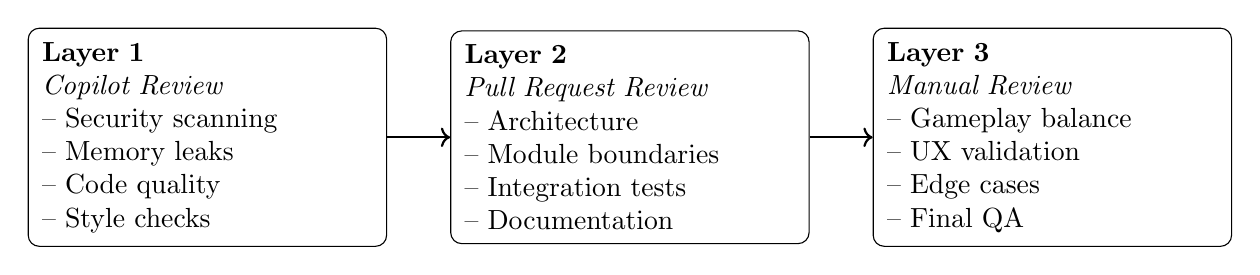
\begin{tikzpicture}[
    node distance=0.8cm,
    layer/.style={
        draw,
        rectangle,
        rounded corners,
        align=left,
        text width=4.2cm,
        inner sep=5pt
    },
    arrow/.style={->, thick}
]

\node[layer] (l1) {
\textbf{Layer 1}\\
\emph{Copilot Review}\\
-- Security scanning\\
-- Memory leaks\\
-- Code quality\\
-- Style checks
};

\node[layer, right=of l1] (l2) {
\textbf{Layer 2}\\
\emph{Pull Request Review}\\
-- Architecture\\
-- Module boundaries\\
-- Integration tests\\
-- Documentation
};

\node[layer, right=of l2] (l3) {
\textbf{Layer 3}\\
\emph{Manual Review}\\
-- Gameplay balance\\
-- UX validation\\
-- Edge cases\\
-- Final QA
};

\draw[arrow] (l1) -- (l2);
\draw[arrow] (l2) -- (l3);

\end{tikzpicture}
\caption{Multi-layer AI-assisted code review process}
\end{figure}


\newpage

\section{Code Quality Achievements}

\subsection{Quality Attributes Achieved}

The final codebase demonstrates exceptional quality across multiple areas including maintainability, robustness and end functionality.

\subsubsection*{Modular Architecture:}
\begin{itemize}
    \item Clear separation of concerns across 7 distinct modules
    \item Well-defined interfaces using header files
    \item Minimal coupling between components
    \item High cohesion within modules
\end{itemize}

\subsubsection*{Code Readability:}
\begin{itemize}
    \item Consistent naming conventions throughout
    \item Appropriate function and variable names
    \item Clear control flow without excessive nesting
    \item Meaningful comments explaining complex logic
\end{itemize}

\subsubsection*{Error Handling:}
\begin{itemize}
    \item Comprehensive input validation
    \item Graceful degradation for missing resources
    \item Proper cleanup in error conditions
\end{itemize}

\subsubsection*{Memory Safety:}
\begin{itemize}
    \item No memory leaks (verified through review)
    \item Proper allocation/deallocation pairing
    \item Bounds checking before array access
    \item Null pointer validation
\end{itemize}

\subsubsection*{Feature Completeness:}
\begin{itemize}
    \item Robust menu system with multiple screens
    \item Comprehensive gameplay mechanics (4 enemy types, 2 aggressive obstacle types, 3 passive obstacles, 4 power-ups)
    \item Persistent ranking system
    \item Full keyboard control scheme
\end{itemize}

\subsubsection*{User Experience:}
\begin{itemize}
    \item Intuitive controls with on-screen guidance
    \item Visual feedback for all player actions
    \item Balanced gameplay difficulty
    \item Engaging enemy behaviors
    \item Dedicated instructions screen
\end{itemize}

\subsection{AI Contribution to Development Efficiency}

The combination of AI velocity and human judgment achieved both speed AND quality---traditionally considered a trade-off. This was possible because:
\begin{enumerate}
    \item AI handled time-consuming mechanical tasks (boilerplate, patterns, documentation)
    \item Human focused on high-value activities (architecture, judgment, testing)
    \item Rapid iteration cycles enabled quick progress without sacrificing quality
    \item Comprehensive AI reviews caught issues early when easy to fix

\end{enumerate}

\newpage

\section{Recommendations for Future Skill Development from AI}

\subsection{Advanced Prompt Engineering}

\subsubsection*{Current Proficiency Level:}
The developer demonstrated good prompt engineering skills, but there is significant room for advancement.

\subsubsection*{Development Opportunities:}

\begin{enumerate}
    \item \textbf{Structured Prompt Templates:}
    \begin{itemize}
        \item Create reusable templates for common development tasks
        \item Include sections for context, requirements, constraints, and success criteria
        \item Develop domain-specific templates (game logic, UI, data structures, etc.)
    \end{itemize}
    
    \item \textbf{Prompt Composition:}
    \begin{itemize}
        \item Learn techniques for building complex prompts from simpler components
        \item Develop hierarchical prompt structures for multi-phase tasks
        \item Practice combining prompts from different AI tools (e.g., ChatGPT $\rightarrow$ Copilot)
    \end{itemize}
    
    \item \textbf{Effective Constraint Specification:}
    \begin{itemize}
        \item Master techniques for specifying code style requirements
        \item Learn to communicate architectural constraints precisely
        \item Practice articulating implicit requirements explicitly
    \end{itemize}
\end{enumerate}

\subsection{Multi-Tool AI Orchestration}

\subsubsection*{Current Proficiency Level:}
The developer successfully orchestrated multiple AI tools but could optimize the workflow further.

\subsubsection*{Development Opportunities:}

\begin{enumerate}
    \item \textbf{Tool Selection Strategy:}
    \begin{itemize}
        \item Develop decision framework for which AI tool to use for each task type
        \item Create a personal ``AI tool matrix'' mapping tasks to optimal tools
        \item Experiment with emerging AI coding assistants (Cursor, Replit Ghostwriter, etc.)
    \end{itemize}
    
    \item \textbf{Workflow Automation:}
    \begin{itemize}
        \item Learn to script repetitive prompt sequences
        \item Explore API-based AI tool integration for custom workflows
        \item Develop templates for common task pipelines
    \end{itemize}
    
    \item \textbf{Cross-Tool Prompt Translation:}
    \begin{itemize}
        \item Master converting prompts between different AI tools' optimal formats
        \item Learn to maintain context across tool transitions
        \item Practice prompt refinement across multiple AI models
    \end{itemize}
\end{enumerate}

\subsubsection*{Practical Exercise:}

Design a complete feature implementation workflow diagram showing:
\begin{itemize}
    \item Which tool handles each phase
    \item What information passes between phases
    \item Decision points for tool selection
    \item Feedback loops for refinement
\end{itemize}

\subsection{Enhanced Testing and Validation}

\subsubsection*{Current Proficiency Level:}
Testing was largely manual, though AI assisted with review. Significant automation opportunities exist.

\subsubsection*{Development Opportunities:}

\begin{enumerate}
    \item \textbf{Test Generation:}
    \begin{itemize}
        \item Learn to prompt AI for comprehensive test case generation
        \item Practice specifying edge cases and boundary conditions
        \item Develop techniques for test oracle generation
    \end{itemize}
    
    \item \textbf{Test Automation:}
    \begin{itemize}
        \item Explore AI-assisted test script generation
        \item Learn to create test data with AI assistance
        \item Practice mocking and stubbing with AI support
    \end{itemize}
\end{enumerate}

\subsubsection*{Recommended Approach:}

After implementing a feature, prompt AI to:
\begin{enumerate}
    \item List all testable behaviors
    \item Generate test cases for each behavior
    \item Identify potential edge cases
    \item Suggest test data for boundary conditions
\end{enumerate}

\subsection{Documentation and Knowledge Management}

\subsubsection*{Current Proficiency Level:}
Good progress logging and README maintenance, with opportunities for more comprehensive documentation.

\subsubsection*{Development Opportunities:}

\begin{enumerate}
    \item \textbf{Automated Documentation:}
    \begin{itemize}
        \item Learn to generate comprehensive API documentation with AI
        \item Practice creating user guides from technical implementations
        \item Develop techniques for maintaining documentation consistency
    \end{itemize}
    
    \item \textbf{Knowledge Extraction:}
    \begin{itemize}
        \item Use AI to extract patterns and principles from code
        \item Practice generating architectural decision records (ADRs)
        \item Learn to create onboarding documentation efficiently
    \end{itemize}
    
    \item \textbf{Documentation Quality:}
    \begin{itemize}
        \item Develop skills in prompting for pedagogical clarity
        \item Practice requesting multiple documentation styles
        \item Learn to generate documentation for different audiences
    \end{itemize}
\end{enumerate}

\subsubsection*{Practical Implementation:}

Create an ``AI Documentation'' custom agent:
\begin{enumerate}
    \item Generate initial documentation from code
    \item Request explanations at different technical levels
    \item Add examples and use cases
    \item Review and refine for clarity
    \item Maintain consistency across updates
\end{enumerate}

\newpage

\section{Experiment: Designing levels with AI}

After the development of Warrior Race Game concluded, an experimental attempt was made to leverage AI tools for level design---a creative domain that proved particularly challenging. This experiment revealed current limitations in AI's capacity for abstract spatial reasoning and gameplay balance intuition.

\subsection{Challenges Encountered}

While AI tools excel at generating semantically correct level files and can populate them with valid entity placements, they lacked the spatial reasoning required for engaging game design. Level design requires understanding how a player will navigate space over time, anticipating movement patterns, and creating rhythms of challenge and relief. These tasks proved beyond current AI capabilities.

\subsubsection*{Lack of Gameplay Flow Understanding}

AI-generated levels were mechanically valid but strategically uninteresting. Entities were placed \textbf{without} consideration for:
\begin{itemize}
    \item Progressive difficulty curves that maintain player engagement
    \item Spatial relationships between obstacles that create meaningful choices
    \item Timing patterns that reward skilled play
    \item Visual composition that guides player attention and movement
\end{itemize}

The generated levels felt arbitrary rather than intentional. Where a human designer might create a ``gauntlet'' section followed by a ``breathing room'' safe zone, AI would distribute challenges randomly, creating tedious gameplay.

\subsubsection*{Inability to Balance Complexity}

A well-designed level balances multiple competing factors: difficulty appropriate to player skill progression, variety to maintain interest, fairness to avoid frustration, and clarity to prevent confusion. AI tools struggled with this multidimensional optimization problem. Prompts addressing one dimension (e.g., ``increase difficulty'') would compromise others (e.g., fairness), requiring iterative refinement that proved inefficient compared to manual design.

\subsection{Prompting Techniques Attempted}

I explored various prompting strategies to overcome these limitations:

\begin{enumerate}
    \item \textbf{Detailed specifications:} Providing explicit entity counts, density parameters, and spacing rules resulted in mechanically correct but creatively bankrupt designs.
    
    \item \textbf{Example-based prompts:} Supplying hand-crafted levels as references yielded slight improvements but mostly produced superficial variations.
    
    \item \textbf{Multi-tool orchestration:} Using ChatGPT for conceptual design and Copilot for implementation provided marginal benefits but couldn't bridge the fundamental creative gap.
\end{enumerate}

\subsection{Time Constraints and Practicality}

Within the experiment's timeframe, achieving satisfactory AI-generated levels proved impossible. The iterative refinement process---identifying deficiencies, crafting corrective prompts, evaluating results---consumed more time than manual level design while producing inferior results. 

A level requiring 30-40 minutes of manual design might demand over 60 minutes of AI-assisted iteration to achieve a similar level of the quality. This shows, that while AI tools provided starting points for human refinement, they were not able to autonomously produce useful  content in this domain.

\newpage

\section{Conclusion}

\subsection{Key Findings}

\begin{enumerate}
    \item \textbf{Workflow Evolution is Essential:}
    \begin{itemize}
        \item AI-assisted development matured significantly over the project lifecycle
        \item The transition from simple autocomplete to orchestrated multi-tool workflows was crucial for maximizing value
        \item Structured processes (PR workflows, explicit prompts, systematic reviews) dramatically improved outcomes
    \end{itemize}
    
    \item \textbf{Quality and Speed Are Compatible:}
    \begin{itemize}
        \item Contrary to traditional trade-offs, AI assistance enabled both rapid development AND high code quality
        \item The key was appropriate division of labor: AI handled mechanical tasks, human focused on judgment and architecture
    \end{itemize}
    
    \item \textbf{Iterative Refinement is Inevitable:}
    \begin{itemize}
        \item Initial AI implementations were rarely complete or perfect
        \item 2--4 refinement cycles per major feature was typical and acceptable
        \item The speed of iteration made this system time-effective overall
    \end{itemize}
    
    \item \textbf{Human Judgment Remains Critical:}
    \begin{itemize}
        \item AI tools struggled with creative, aesthetic, and balance decisions
        \item Final quality depended on effective human review and refinement
        \item The most successful outcomes combined AI capability with human expertise
    \end{itemize}
    
    \item \textbf{Context and Communication Matter:}
    \begin{itemize}
        \item Quality of AI output was directly proportional to prompt quality
        \item Explicit communication of requirements, constraints, and style preferences was essential
        \item Use of other AI tools for prompt refinement significantly improved code implementation quality
    \end{itemize}
\end{enumerate}

\subsection{Project Success Factors}

The project achieved exceptional outcomes due to several factors:

\begin{enumerate}
    \item \textbf{Clear Vision:}
    \begin{itemize}
        \item Well-defined goals and success criteria
        \item Strong architectural instincts guiding AI implementation
        \item Consistent quality standards throughout
    \end{itemize}
    
    \item \textbf{Appropriate Tool Selection:}
    \begin{itemize}
        \item Use of specialized AI tools for different tasks
        \item Recognition of each tool's strengths and weaknesses
        \item Willingness to try multiple approaches
    \end{itemize}
    
    \item \textbf{Systematic Review:}
    \begin{itemize}
        \item Multi-layered review processes catching different issue types
        \item Integration of AI and manual review complementarily
        \item Continuous quality assurance rather than end-of-project testing
    \end{itemize}
    
    \item \textbf{Learning and Adaptation:}
    \begin{itemize}
        \item Continuous refinement of AI collaboration workflows
        \item Documented learning (progress log) enabling reflection
        \item Willingness to adjust approaches based on outcomes
    \end{itemize}
\end{enumerate}

\subsection{Final Reflection}

The Warrior Race Game project exemplifies the potential of thoughtful human-AI collaboration in software development. The student successfully:

\begin{itemize}
    \item Leveraged AI tools to significantly accelerate development and the learning curve
    \item Maintained high code quality through systematic review processes
    \item Achieved rapid feature iteration while preserving architectural integrity
\end{itemize}

The project's success was not due to AI replacing human judgment, but rather to AI amplifying human capabilities. \textbf{The student maintained strong architectural vision}, made critical design decisions, ensured gameplay balance, and provided the direction that shaped the final product. \textbf{AI tools accelerated implementation}, improved consistency, caught errors early, and \textbf{enabled rapid iteration.}

This synthesis of human expertise and AI capability represents the future of software development: \textbf{human and AI working in a partnership}. The students who master this collaboration will be far more effective than either human or AI working alone.

\newpage

\end{document}